\documentclass{beamer}
\usetheme[titlepagelogo=logounipd,% Logo for the first page
		  language=italian,
		  bullet=triangle,
		  color=green,
         ]{TorinoTh}
        

\usepackage[beamer,customcolors]{hf-tikz}
\usepackage{tikz}
\usepackage{color, colortbl}

\definecolor{ARow}{rgb}{1,.8,.8}
\definecolor{BRow}{rgb}{1,.6,.6}


\hfsetfillcolor{alerted text.fg!10}
\hfsetbordercolor{alerted text.fg}

\author{Alberto Andeliero}
\rel{Prof. Tullio Vardanega}
\title[Recommendation system]{Recommendation system}
\ateneo{Universit\`{a} degli Studi di Padova}
\date{14 Aprile 2016}

\usepackage{amsmath,amssymb,amsfonts,amsthm}
\usepackage{bigints}
\usepackage{bookmark}
\usepackage{booktabs}
\usepackage{emptypage}
\usepackage{array} % needed for \arraybackslash
\usepackage{graphicx}
\usepackage{adjustbox} %\includegraphics{figura.ext}
\usepackage{epstopdf} % per includere immagini .eps
\usepackage{subfig}
\usepackage{quoting}
\usepackage{listings}
\usepackage{bm}
\usepackage{eurosym}
%\usepackage{enumerate}
%\usepackage{enumitem}
%\usepackage{fourier} % font figo
%\usepackage{euler}
%\usepackage{microtype}

\newcommand{\N}{\mathbb{N}}
\newcommand{\Z}{\mathbb{Z}}
\newcommand{\Q}{\mathbb{Q}}
\newcommand{\R}{\mathbb{R}}
%\newcommand{\C}{\mathbb{C}}
\newcommand {\matlab} {$\text{Matlab}^{\circledR}$\,}
\newcommand {\expect} {\mathbb{E}}
\newcommand {\prob} {\mathbb{P}}
\renewcommand{\epsilon}{\varepsilon}
\renewcommand{\theta}{\vartheta}
%\renewcommand{\sigma}{\varsigma}

% Teoremi, definizioni, etc
\theoremstyle{definition}
%\newtheorem{definition}{Definition}
\newtheorem{eg}{Example}
\newtheorem{characterization}{Characterization}

\theoremstyle{plain} 
%\newtheorem{theorem}{Theorem}
\newtheorem{proposition}[theorem]{Proposition}
%\newtheorem{corollary}[theorem]{Corollary}

\theoremstyle{remark}
\newtheorem{remark}{Remark}

% Codice matlab
%\usepackage{mcode}
%\lstset{basicstyle=\small\ttfamily}
%\lstset{language=Matlab}

% Immagini
\graphicspath{{img/}}



\begin{document}
\titlepageframe % Specific command 

\begin{frame}
\frametitle{Indice}
\begin{itemize}
\item \textbf{Presentazione azienda}
\item \textbf{Il progetto nella strategia aziendale}
\item \textbf{Il progetto di stage}
\item \textbf{Resoconto}
\end{itemize}
\end{frame}


%Primo capitolo
\begin{frame}
\frametitle{L'azienda}
\begin{minipage}[c]{.45\textwidth}
\centering 

\includegraphics[width=\textwidth]{slide1}
\end{minipage}
\begin{minipage}[c]{.45\textwidth}
Prodotti e servizi:
\begin{itemize}
\item E-commerce
\item Knowledge management system
\item Servizio clienti
\item Web-marketing
\end{itemize}
%I linguaggi e i framework glieli dico a voce
\end{minipage}
\end{frame} %L'azienda (+ prodotti e servizi, + tecnologie di riferimento)
\begin{frame}
\frametitle{Processi aziendali e strumenti}
\begin{minipage}[c]{.55\textwidth}
\centering 
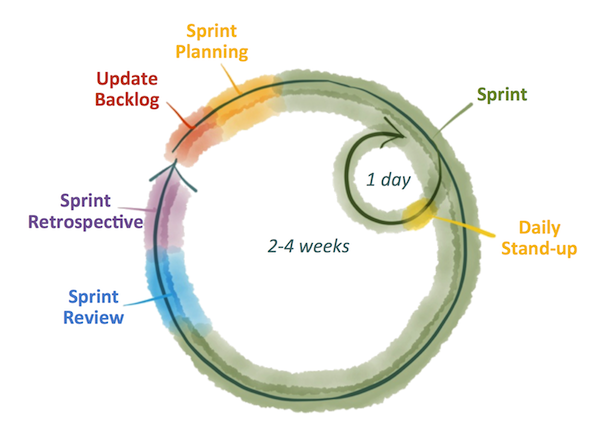
\includegraphics[width=\textwidth]{scrumccarino}
\end{minipage}
\begin{minipage}[c]{.35\textwidth}
Strumenti utilizzati
\begin{itemize}
\item Zendesk
\item Jira e Scrum Board
\item Google Docs
\item Git
\item Sublime text e Eclipse
\item Windows e MacOS
\end{itemize}
\end{minipage}
\end{frame}
 %Processi aziendali e strumenti

%Secondo capitolo
  
\begin{frame}
\frametitle{Progetto}
\begin{minipage}[b][0.5\textheight][t]{\textwidth}
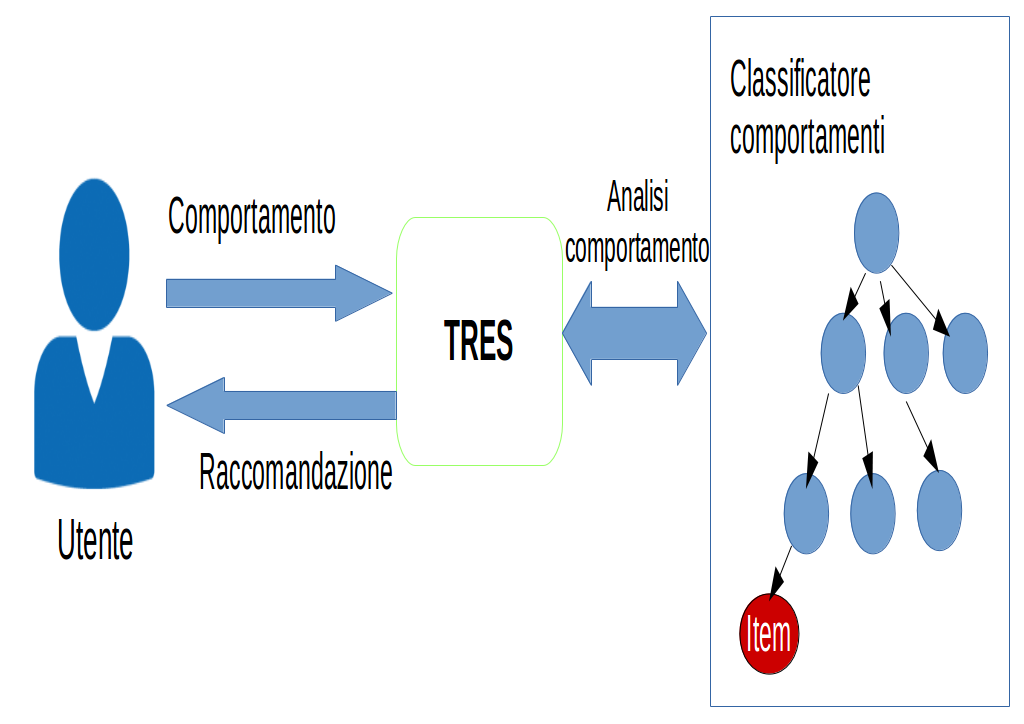
\includegraphics[height=100pt, width=\textwidth]{sistemadiracc}
\end{minipage}
\begin{minipage}[b][0.5\textheight][t]{\textwidth}
\begin{alertblock}{Obiettivo}
Realizzazione di un sistema di raccomandazione\\ basato sul comportamento utente
\end{alertblock}
\end{minipage}
\end{frame} %Il progetto nella strategia aziendale
\begin{frame}[t]
\frametitle{Vincoli}
\begin{minipage}[t]{.31\textwidth}
Temporali
\begin{itemize}
\item[]
\item[]
\item[] \textbf{300 ore}
\begin{itemize}
\item[] 37.5 ore settimanali
\end{itemize}
\end{itemize}
\end{minipage}
\vrule{}
\begin{minipage}[t]{.32\textwidth} 
Metodologici
\begin{itemize}
\item[] 
\includegraphics[width=0.50\textwidth]{img/sbt-logo}
\item[] 
\includegraphics[width=0.50\textwidth]{img/intellij-logo}
\item[] 
\includegraphics[width=0.66\textwidth]{img/astah-logo}
\item[] 
\includegraphics[width=0.50\textwidth]{img/travisci-logo}
\item[] 
\includegraphics[width=0.50\textwidth]{img/git-logo.jpg}
\end{itemize}
\end{minipage}
\vrule{}
\begin{minipage}[t]{.32\textwidth}
Tecnologici
\begin{itemize}
\item[] 
\includegraphics[width=0.66\textwidth]{img/scala-logo}
\item[] 
\includegraphics[width=0.66\textwidth]{img/play-logo}
\item[] 
\includegraphics[width=0.66\textwidth]{img/orientdb-logo}
\end{itemize}
\end{minipage}
\end{frame} %Obiettivi e vincoli

%Terzo capitolo
\begin{frame}
\frametitle{Analisi dei requisiti}
UC1 Utilizzo di API per le raccomandazioni
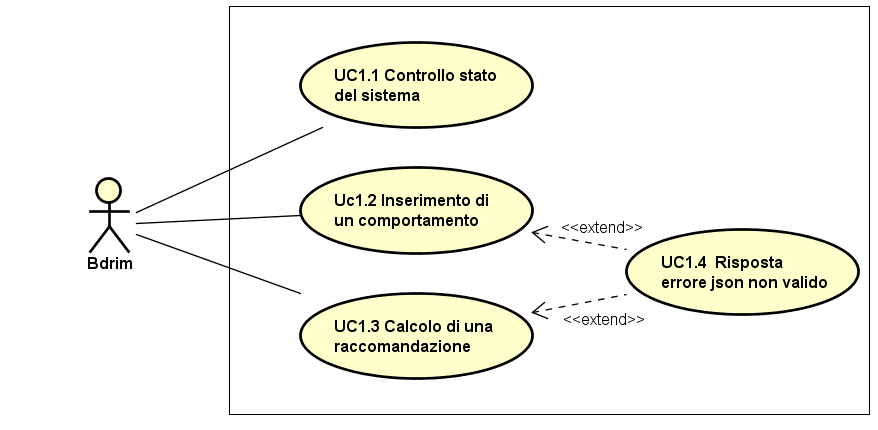
\includegraphics[width=\textwidth]{uc1}
\end{frame} %qui ci metto il caso d'uso UC1
\begin{frame}
\frametitle{Visione generale}

\begin{minipage}[c]{.60\textwidth}
\centering 
\includegraphics[width=\textwidth]{visgen}
\end{minipage}
\begin{minipage}[c]{.38\textwidth}

\begin{itemize}
\item[ROUTER] Componente di Play
\begin{itemize}
\item Convoglia le richieste HTTP al controller
\end{itemize}
\item[CLIENT] Bdrim
\begin{itemize}
\item Piattaforma di raccolta dati
\end{itemize}

\item[SERVER] Tres
\begin{itemize}
\item Sistema di raccomandazione
\end{itemize}
\end{itemize}
\end{minipage}
\end{frame} %qui ci metto l'immagine generale
\begin{frame}
\frametitle{Modellazione databse}
\begin{minipage}[t][0.4\textheight][t]{\textwidth}
\includegraphics[width=\textwidth]{databaseschema}
\end{minipage}
\begin{minipage}[b][0.6\textheight][t]{\textwidth}
   \begin{itemize}
	\item \textbf{Property graph}
	\begin{itemize}
		\item I vertici sono entità
		\item Gli spigoli sono relazioni
	\end{itemize}	 
    \item \textbf{Schema-full}
   \end{itemize}
\end{minipage}
\end{frame} %slide sulla modellazione
\begin{frame}
\frametitle{Architettura}
\begin{minipage}[c]{.38\textwidth}
Design pattern
\begin{itemize}
\item MVC
\item DAO
\item Strategy
\item Singleton
\end{itemize}
\end{minipage}
\begin{minipage}[c]{.60\textwidth}
\centering 
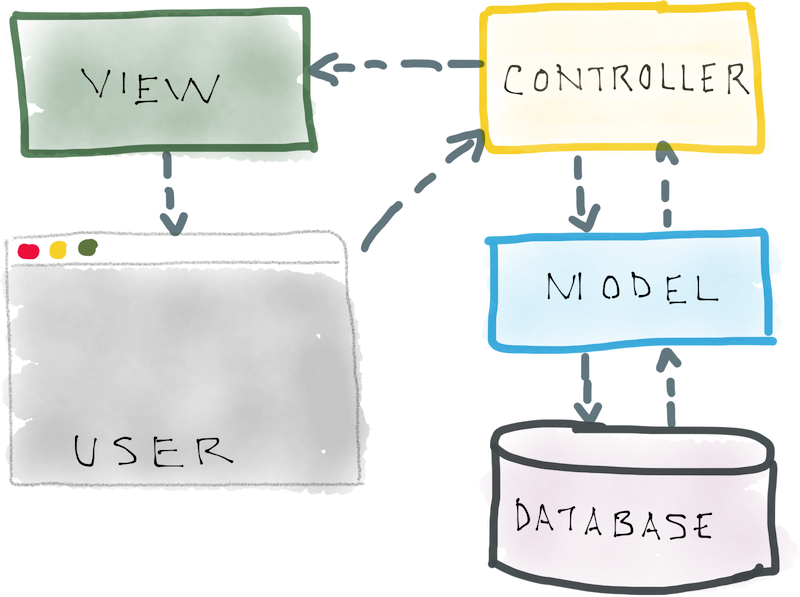
\includegraphics[width=\textwidth]{mvc}
\end{minipage}
\end{frame} %package mvc e un elenco dei pattern utilizzati
\begin{frame}
\frametitle{Strumenti e metriche}
\begin{minipage}[c]{.45\textwidth}
\begin{itemize}
\item[] 
\includegraphics[width=0.7\textwidth]{intellij-logo}
\item[] 
\includegraphics[width=0.7\textwidth]{specs2}
\item[] 
\includegraphics[width=0.7\textwidth]{codecov}
\end{itemize}
\end{minipage}
\begin{minipage}[c]{.45\textwidth}
Metriche adottate
\begin{itemize}
\item Complessità ciclomatica
\item Attributi per classe
\item Densità commenti
\item Copertura dei test
\end{itemize}
\end{minipage}


\end{frame} %presento gli strumenti utilizzati e le metriche che sono andato a rilevare
%\input{cap/funzionamento.tex} %procedura di raccomandazione
\begin{frame}
\frametitle{Risultati}


\begin{minipage}[t][0.50\textheight][t]{\textwidth}
\textbf{Metriche}\\
\begin{tabular}{lccc}
\rowcolor{BRow}						    &	Range		& Misurato 		 & Esito \\
\rowcolor{ARow} Complessità ciclomatica & \textless 10	& \textless 10	 & positivo \\
\rowcolor{BRow} Attributi per classe    & 1-8 			& max 4 e avg 2  & positivo \\
\rowcolor{ARow} Copertura commenti 	    & 80\% - 100\%  & 100\%  		 & positivo \\
\rowcolor{BRow} Copertura dei test 	    & 70\% - 100\%  & 73\%  		 & positivo \\
\end{tabular}
\end{minipage}
\begin{minipage}[b][0.50\textheight][t]{\textwidth}
\textbf{Test}
\begin{itemize}
\item Unità 10/10
\item Integrazione 3/3
\item Sistema 3/3
\end{itemize}
\end{minipage}





\end{frame}
%Quarto capitolo
\begin{frame}
\frametitle{Bilancio sui risultati}

\begin{minipage}[c]{.45\textwidth}
\centering 
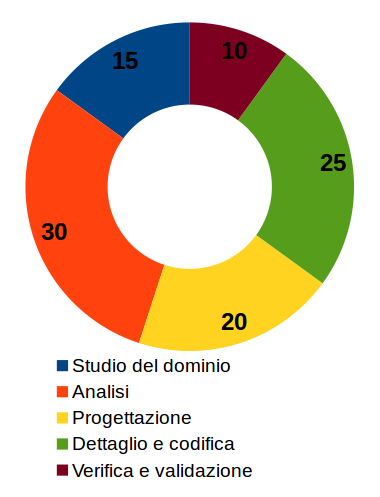
\includegraphics[height=0.7\textheight]{impegnoperc}
\end{minipage}
\begin{minipage}[c]{.45\textwidth}
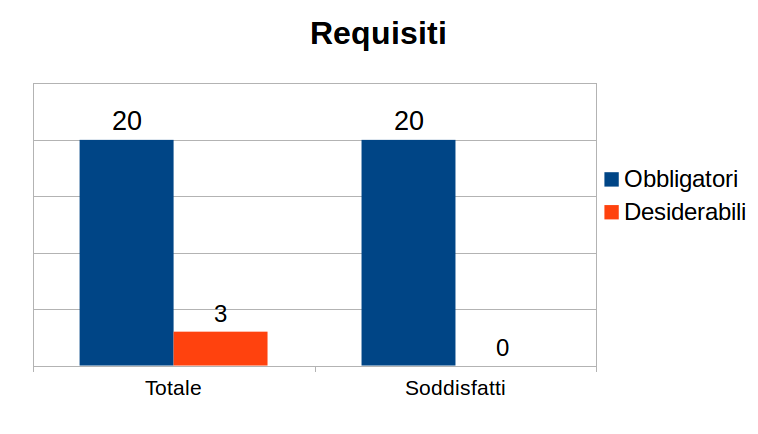
\includegraphics[height=0.4\textheight]{graficorequisiti}\\
Traguardi
\begin{itemize}
\item Tecnologie innovative
\item Gestione di progetto
\item Team working
\end{itemize}
\end{minipage}


%\begin{minipage}[c]{.45\textwidth}

%\end{minipage}

\end{frame} %Bilancio risultati









%\input{chap/intro.tex}
%\input{chap/filter.tex}
%\input{chap/ML.tex}
%\input{chap/gibbs.tex}
%\input{chap/experiment.tex}
%\input{chap/theend.tex}

\end{document}





%
%\begin{frame}[t,fragile]{Configurazione}
%\begin{itemize}
%\item La configurazione di questo tema è:
%\begin{itemize}
%\item \verb!language=italian!
%\item \verb!coding=utf8x!
%\item \verb!titlepagelogo=name-of-the-logo!
%\item \verb!bullet=triangle!
%\item \verb!color=green!
%\end{itemize}
%\item La maggior parte delle opzioni, effettivamente tutte a parte \highlight{titlepagelogo}, può essere omessa utilizzando il tema standard
%\end{itemize}
%\end{frame}
%
%\begin{frame}[fragile]{Comportamento degli alert}
%Scegliendo un colore, il tema evidenzia il testo di conseguenza. Per inserire gli alert nell'ambiente \emph{itemize}, potete utilizzare:
%\begin{verbatim}
%\begin{itemize}
%\item<+-| alert@+> Mela
%\item<+-| alert@+> Pesca
%\end{itemize}
%\end{verbatim}
%Ad esempio:
%\begin{itemize}
%\item<+-| alert@+> Mela
%\item<+-| alert@+> Pesca
%\end{itemize}
%\end{frame}
%
%\begin{frame}[fragile]{Un diverso approccio per evidenziare il testo}
%Se volete evidenziare il vostro testo al di fuori dell'ambiente \emph{itemize}, Beamer2Thesis offre le seguenti possibilità:
%\begin{itemize}
%\item il comando standard \verb!\alert{testo}!: evidenzia semplicemente il vostro \alert{testo}
%\item il comando \verb!\highlight{testo}!: evidenzia il vostro \highlight{testo} rendendolo corsivo
%\item il comando \verb!\highlightbf{testo}!: evidenzia il vostro \highlightbf{testo} in grassetto
%\end{itemize}
%Ovviamente, il colore utilizzato è quello da voi scelto nel preambolo.
%\end{frame}
%
%\begin{frame}[fragile]{Evidenziare formule matematiche}
%\begin{itemize}
%\item Il pacchetto \href{http://www.ctan.org/pkg/hf-tikz}{hf-tikz} permette di evidenziare formule matematiche (completamente o in parte) in Beamer con animazioni semplici 
%\item Si possono adattare i colori del tema così:
%\begin{verbatim}
%\usepackage[beamer,customcolors]{hf-tikz}
%\hfsetfillcolor{alerted text.fg!10}
%\hfsetbordercolor{alerted text.fg}
%\end{verbatim}
%\item È necessario \highlight{compilare due volte} per ottenere il risultato voluto!
%\item Si legga la documentazione del pacchetto per ulteriori opzioni; un esempio di utilizzo è riportato nella diapositiva successiva.
%\end{itemize}
%\end{frame}
%
%\begin{frame}[fragile]{Evidenziare formule matematiche (II)}
%\begin{itemize}
%\item Esempio:
%\[\tikzmarkin<2->{a}x+\tikzmarkin<1>{b}y\tikzmarkend{b}=10\tikzmarkend{a}\]
%\item<2-> Codice:
%\begin{verbatim}
%\[\tikzmarkin<2->{a}x+
%  \tikzmarkin<1>{b}y\tikzmarkend{b}
%  =10\tikzmarkend{a}\]
%\end{verbatim}
%\end{itemize}
%\end{frame}
%
%\begin{frame}[t,fragile]{Il risultato}
Il pdf generato presenta, automaticamente, alcune proprietà:
\begin{itemize}
\item il titolo
\item il nome dell'autore
\item l'oggetto
\begin{itemize}
\item Thesis Presentation utilizzando la lingua inglese
\item Presentazione Tesi di Laurea in italiano
\end{itemize}
\end{itemize}
Tutto ciò è reso possibile grazie alle opzioni del pacchetto hyperref. Per creare riferimenti nel testo il codice da utilizzare è:
\begin{itemize}
\item \verb!\label{nome-riferimento}! nel punto sorgente
\item \verb!\ref{nome-riferimento}! nel punto in cui richiamate il riferimento
\item \verb!\href{url}{name-url}! per specificare indirizzi web
\end{itemize}
\end{frame}


\begin{frame}[fragile]{Suggerimenti}
\begin{itemize}
\item Per realizzare una slide si usa l'ambiente \emph{frame}, con allineamenti in alto (t), al centro (c) oppure in basso (b): suggerisco di usare il primo; il codice è\\
\verb!\begin{frame}[t]{titolo-della-slide}!
\begin{flushleft}
text
\end{flushleft}
\verb!\end{frame}!
\item Per facilitare la scrittura ho creato un nuovo ambiente che ha questa proprietà intrinsecamente:\\
\verb!\begin{tframe}{titolo-della-slide}!
\begin{flushleft}
text
\end{flushleft}
\verb!\end{tframe}!
\end{itemize}
\end{frame}

\begin{frame}[fragile]{Suggerimenti (II)}
\begin{itemize}
\item Per realizzare la prima pagina, è stato introdotto il comando \verb!\titlepageframe!
\begin{itemize}
\item naturalmente è possibile usare un approccio più \emph{standard}\\
\verb!\begin{frame}[plain]!\\
\verb!\titlepage! \\
\verb!\end{frame}!
\item In questo caso \textbf{non} inserite un titolo alla slide
\end{itemize}
\item Se dovete inserire del codice con gli ambenti \emph{verbatim} o \emph{listings} \textbf{non utilizzate} \emph{tframe}, ma:\\
\verb!\begin{frame}[t,fragile]{titolo-della-slide}!
\begin{verbatim}
\verb!codice!
\end{verbatim}
\verb!\end{frame}!
\end{itemize}
\end{frame}

\begin{frame}[t,fragile]{Suggerimenti (III)}
\begin{itemize}
\item Se il titolo è troppo lungo rischia di non essere perfettamente inserito a fondo diapositiva, perciò si può utilizzare il \highlight{titolo corto}; ad esempio:
\begin{verbatim}
\title[Titolo corto]{Titolo lungo}
\end{verbatim}
In questo modo il titolo lungo viene soltanto inserito nel frontespizio.
\item In caso si abbiano più di due relatori o correlatori, suggerisco di inserirli con i comandi riportati in slide \ref{secondrel} separati da una virgola.
\end{itemize}
\end{frame}

\begin{tframe}{Su Facebook}
La rilevanza di Facebook, ad oggi, è nota a tutti: per questo motivo, esistono:
\begin{itemize}
\item il gruppo \href{https://www.facebook.com/\#!/groups/beamer2thesis/}{Beamer2Thesis}
\item la pagina \href{https://www.facebook.com/\#!/pages/Beamer2Thesis/112814205489099}{Beamer2Thesis}
\end{itemize} 
In questo modo potete postare i vostri commenti, suggerimenti, idee e domande in modo più \emph{familiare}. Inoltre è possibile trovare ulteriori esempi.
\end{tframe}

\begin{tframe}{Cronologia}
Di seguito sono riportate le principali caratteristiche delle versioni:
\begin{itemize}
\item iniziale (2011-01-17):
\begin{itemize}
\item colori, secondo logo, secondo candidato, ambiente tframe, titleline, bullet, lingue (inglese, italiano), separatore per la numerazione delle slide; 
\end{itemize}
\item versione 2.0:
\begin{itemize}
\item terzo logo, correlatore, nuovi modi di evidenziazione del testo, comando per il frontespizio, nuovi ambienti \emph{adv} e \emph{disadv}, supporto a \XeTeX\, e \XeLaTeX\,, ambienti block;
\end{itemize}
\item versione 2.1:
\begin{itemize}
\item opzione sulla codifica, secondo relatore, secondo correlatore.
\end{itemize}
\item versione 2.2:
\begin{itemize}
\item supporto per più lingue, titolo corto, suggerimento per evidenziare formule matematiche.
\end{itemize}
\end{itemize}
\end{tframe}

\begin{tframe}{Ringraziamenti}
\begin{itemize}
\item Voglio ringraziare le persone, che con preziosi suggerimenti, hanno contribuito alla realizzazione:
\begin{itemize}
\item Alessio Califano
\item Alessio Sanna
\item Luca De Villa Palù
\item Mariano \emph{Dave} Graziano
\item Giovanna Turvani
\item Mattia Stefano
\item Nicola Tuveri
\item Giuliana Galati
\end{itemize}
\end{itemize}
Un ringraziamento speciale è per il professor Claudio Beccari per i commenti sulla prima versione.
\end{tframe}